\documentclass[pageno]{jpaper}

% Change to current semester and year, e.g.:
% \newcommand{\IWreport}{Spring 2020}
\newcommand{\IWreport}{Spring 2023}
\newcommand{\quotes}[1]{``#1''}


\widowpenalty=9999

\usepackage[normalem]{ulem}
\usepackage{algpseudocodex}
\usepackage{algorithm}
\usepackage{amsfonts}
\usepackage{amsmath}

\begin{document}

\title{A Visual Modeling Tool for Trajectory Planning for Autonomous Quadrotors}

\author{Arti Schmidt \\ Adviser: Zachary Kincaid}

\date{}
\maketitle

\thispagestyle{empty}
\doublespacing
\begin{abstract}
Quadcopters are one of the most widely used classes of flying robots. Their ability to perform complex maneuvers at speeds ranging from a hover to 100kph while carrying a payload of computers and sensors has made them a popular platform for a variety of applications including cinematography, inspection, and even sport in the form of drone racing. Increasingly powerful autonomous capabilities has made them more accessible for these and other applications in recent years. Autonomous flight is often split into the tasks of perception, planning, and control. The planning component refers to the generation of a path through the environment that a quadcopter will track during its flight. There is extensive literature on trajectory planning methods for quadcopters, and a recent paper proposed a visual modeling system for 2D trajectories, but the restriction to 2D prevents taking full advantage of quadcopter capabilities. In this work, a 3D visual modeling system is developed which allows humans to specify constraints via an intuitive interface that a trajectory planning algorithm can use to generate trajectories satisfying some objective. This work will focus on time optimal trajectories, as would be desired in a drone racing context. Constraints can be of various types, including waypoints for a drone to pass through, keep out regions defined by 3D meshes, and speed or altitude thresholds. Several trajectory planning algorithms, including those based on polynomial representations, optimization over discrete time steps, and neural networks, will be evaluated and compared in simulation. Specifically, a drone’s ability to accurately track the generated trajectories and their completion time will be measured.
\end{abstract}

\section{Motivation}

This project’s aim is to build a tool that allows users to model these types of trajectories for use by autonomous quadrotors
What is a quadrotor
Trajectories recorded from a camera on the drone

Robots are becoming increasingly prevalent in modern society because they can perform many monotonous tasks faster, safer, and more reliably than humans, and allow people to spend their time in better ways. As robotics and the AI that powers them becomes more advanced, they are able to accomplish higher level and more open ended tasks that previously were only possible with human decision making power.

Drones are a ubiquitous type of robot today. They are extremely versatile, and can do everything from hovering to cruising at speeds well over 100 kph, accelerate at 4 g, perform inverted acrobatic maneuvers, and operate in both cluttered urban environments and wide open landscapes. Their wide range of flight capabilities have led to applications in videography, inspection, search and rescue, and many others, plus the creation of activities centered around the drones themselves, like drone racing and freestyle flight, which are done for entertainment and competition. As drones have become increasingly powerful and valuable for various industries, their level of autonomy has also increased to match. Pilots can now rely on features like obstacle avoidance, autonomous flight between waypoints, and ???, while new possibilities like flight in areas without signal or at long distances with high latency, and repetitive tasks like package delivery are also created.

Freestyle flight is a popular activity for drone hobbyists, in which the pilot showcases their ability or the beauty of the surroundings. Freestyle flight is quite a general term that can encompass many styles of flight, including everything from rapidly dodging obstacles in an indoor environment and diving alongside buildings to long range flight along mountainsides and cruising just above bodies of water. As such, it is not easy to precisely define the qualities that comprise freestyle flight. ? something more about this *which makes it challenging to generally represent these kinds of flights*?

Like many other applications of drones, freestyle flight has historically been squarely in the domain of human pilots, especially because it is in many ways an artistic endeavor that requires both high level decision making to create an interesting and entertaining flight plan, as well as low level piloting skill to make the flight look good. It is not immediately clear whether adding any amount of autonomy to this formula could be beneficial or desirable at all. While this may indeed be an activity where humans will not be surpassed by computers for the foreseeable future, there are certainly situations in which computers may be useful for this purpose. For example, consider shooting a scene for a movie which may require precisely planned movements or a high degree of repeatability to do multiple takes. Or, a pilot may be unavailable or too expensive to hire for a small project. Or, the flight may involve being between obstacles at long range, where a loss of signal and crash would be likely for a human pilot. Having the ability to do autonomous freestyle flight would be invaluable in all of these cases, and as they suggest, freestyle flight can be more than just a form of entertainment. Finally, the complex and open-ended nature of freestyle flight makes it a great way to demonstrate and test the state of the art in AI and drone technology as it becomes ever more humanlike.

What is the project and why is it useful for people to have?

\section{Background}

How does motion planning fit with other aspects of autonomous flight?
How is my project different from both of the in depth mentioned papers?
Exactly what about the constraints makes them good for freestyle trajectories? (rotation)

Add math notation?

A trajectory is a continuous function that gives the position and rotation of a quadrotor in R3 at any given time. ??feasible trajectory?? ??there are many trajectories between two points?? Trajectory planning for quadrotors is a hard problem because the state space is both large and high dimensional. The quadrotor’s state includes position in R3, velocity in R3, and rotation in SE(3), for a total of nine dimensions [CITATION]. And in some applications, trajectories may be planned over distances of many kilometers, while requiring a resolution on the order of centimeters in some locations to navigate around obstacles. Furthermore, a trajectory must be feasible, meaning that it respects the quadrotor dynamics. Specifically, the amount of linear and angular acceleration that a quadrotor can produce is limited, and additional considerations like aerodynamic drag also exist for more complicated quadrotor models. And finally, many additional constraints may be imposed on a trajectory, such as position constraints to ensure that the quadrotor does not pass through obstacles, or speed constraints to ensure that the quadrotor does not exceed a maximum speed in some segment.

Many methods for planning quadrotor trajectories have been proposed in the literature. These include global optimization approaches, sampling methods, and leveraging polynomial representations of trajectories ?add more detail, specifically min snap generation? [CITATION]. Many of these methods are concerned with generating time optimal and collision free trajectories, which are useful in the context of drone racing, for example. Some methods also consider other objectives, like finding the trajectory that will best keep important landmark objects in view [CITATION]. ?As mentioned previously?, the objective function for freestyle trajectories is challenging to define. Move this to approach section: *need smoothness, don’t care about speed, any trajectory that satisfies constraints is fine*

To the author’s knowledge, trajectory planning for freestyle flight has not explicitly been considered before in the literature, but as noted, freestyle flight is a term with fairly broad applicability and could be used to describe many types of flight trajectories.

One widely cited work on quadrotor trajectory generation by Mueller et al. [CITATION] proposed a method for generating “motion primitives”, which are essentially simple trajectories that can be used as building blocks for creating more complex ones. A motion primitive is constrained by the quadrotor’s initial and final position, velocity, and acceleration, as well as the flight duration. The final translational variables may also be left free in any dimensions. Motion primitives are fifth degree polynomial trajectories that are chosen to minimize the squared norm of their jerk while respecting the initial and final constraints. Jerk refers to the first derivative of acceleration, and as Mueller et al. explain, this cost function is “representative of the aggressiveness of the true system inputs” [CITATION]. This is because the control inputs are the rotor speeds, which are directly related to the quadrotor’s linear and angular acceleration, and so minimizing the jerk corresponds to minimizing the change in these accelerations, and thus also roughly minimizing the control inputs. The paper derives a closed form solution for generating these motion primitives by deferring feasibility testing to a later step (instead of incorporating these constraints into the optimization problem), and solving for each spatial dimension independently [CITATION]. By doing so, generating motion primitives just requires evaluating a matrix multiplication along each axis. Feasibility of the motion primitive is determined by comparing the required thrust and body rates to the user supplied minimum thrust and maximum thrust and body rates. This test is applied recursively along the motion primitive with increasingly short time intervals. With this approach, “on the order of one million motion primitives per second can be generated and tested for feasibility on a laptop computer with an unoptimized implementation” [CITATION], which makes it ideal for searching over many final constraints and durations to find the motion primitive which best achieves the goal [CITATION]. Mueller et al. provide both a Python and C++ implementation of their method. This project relies heavily on the ideas presented in their paper as well as their implementation, which will largely be treated as a black box for the rest of this paper. [ADD MORE DETAIL BEHIND METHOD?]

[PAPER PRIMITIVE VISUALIZATION GRAPH]

In addition to trajectory generation, this project also addresses the creation of a user interface for defining trajectory constraints and visualizing the resulting trajectory. This aspect of the project was inspired by a visual modeling tool for 2D trajectories created by Mceowen et al. [CITATION]. In their paper, they describe and implement an optimization based approach to trajectory generation that uses successive convexification, which has had demonstrated success in applications ranging from quadrotors to rocket landing [CITATION]. As they explain, formulating a problem so that this method can be applied takes a significant amount of work and knowledge of the theory, which makes it unapproachable for a typical user that would like to be able to simply specify a trajectory. To fix this, they create a visual modeling system that gives users a graphical interface for defining constraints and providing information about the resulting trajectory. Users can define positional constraints, elliptical keep out zones, and constraints like slow zones that are active only when the quadrotor is in a certain set of states. [EMPHASIZE 2D]

\section{Approach}

In this project, the constraints for a trajectory are given as $C_i = (x_i, R_i, t_i)$ for all $i \in \{1, \dots, n\}$, where $n$ is variable. Constraint $C_i$ requires that the quadrotor is at position $x_i \in \mathbb{R}^3$, $t_i \in \mathbb{R}_{\geq 0}$ seconds after arriving at $x_{i-1}$. That is, $t_i$ is the flight time between $x_{i-1}$ and $x_i$, and $t_1$ is arbitrary as the quadrotor's initial position is assumed to be $x_1$. Optionally, $R_i \in SO(3)$ can be specified, which requires that the quadrotor has rotation matrix $R_i$ at $t_i$. An unconstrained rotation is denoted as $\emptyset$. Note that the trajectory generation algorithm ignores rotation about the quadrotor's yaw axis, which is discussed later. This choice of constraints should allow for the specification of a diverse range of trajectory styles, such as the trajectories found in freestyle flight. For simplicity, constraints describing keep out regions (to avoid obstacles, for example) are not supported. Instead, users can set position constraints as necessary until the generated trajectory does not intersect any of these regions. The sequence of position constraints determines the basic structure or route that the trajectory will take, which could be on the scale of meters or kilometers. Duration constraints affect the quadrotor's speed. Rotation constraints allow for controlling the direction of the quadrotor's camera and specifying acrobatic maneuvers like inversions. A trajectory for flying along a mountain ridge may only require a simple sequence of position constraints with arrival times set to achieve the desired speed. On the other hand, a trajectory for flying between buildings and other urban obstacles while performing acrobatics could make use of many position constraints to ensure that the generated trajectory closely follows a desired path, as well as rotation constraints to, for example, point downwards while diving alongside a building, keep a sculpture in view while flying around it, or be upside down when at the apex of a loop.

To generate trajectories that respect these constraints, an algorithm is developed which builds on the motion primitive library from Mueller et al. It works by reducing the generation of the full trajectory to generating a sequence of motion primitives with appropriate initial and final constraints using a greedy heuristic. This approach is chosen from among the many options described in the literature because motion primitives are simple and understandable, and the paper provides an easy to use Python implementation for generating them. Additionally, they can be made to work with the constraint model described above without modification to the underlying approach, and their optimization objective of minimal jerk is a good choice for freestyle trajectories. As mentioned previously, trajectories for freestyle flight do not need to be optimal with respect to time or any other easily apparent metric, they need only respect the given constraints. However, to the extent possible, freestyle trajectories should appear relatively smooth and natural, which makes them more enjoyable and engaging to watch. Again, this is a challenging objective to formalize, but one possibility is to minimize some derivative of the quadrotor's position with respect to time. Because jerk roughly corresponds to the aggressiveness of the inputs to the quadrotor [CITATION], it is a sensible choice for producing trajectories that look smooth. Unfortunately, the motion primitive library does lack one important feature, which is the generation of yaw angle trajectories [CITATION]. The quadrotor yaw angle can be considered independently of the other inputs since it is rotation about the thrust axis, and thus it is a sensible omission from the library. But, a yaw trajectory is essential for freestyle flight in particular, because this controls where the camera points, and so it is necessary for visually appealing camera footage from onboard the drone. While generating yaw trajectories could likely be a straightforward addition for this project, this was not done due to time constraints, and so the quadrotor's yaw angle is always fixed at zero. The following notation is used regarding motion primitives for the rest of this paper. $g(p_0, v_0, a_0, p_1, v_1, a_1, t)$ is the motion primitive generation function, which takes parameters, in order, for the quadrotor initial position, velocity, and acceleration; final position, velocity, and acceleration; and the motion primitive duration. It returns a trajectory object $\tau$ using Mueller et al.'s algorithm, or the value $\emptyset$ if this is infeasible. $x_{\tau}(t)$, $\dot x_{\tau}(t)$, $\ddot x_{\tau}(t)$, and $R_{\tau}(t)$ are functions which query for the quadrotor position, velocity, acceleration, and rotation, respectively, at a given time $t$ along trajectory $\tau$.

\begin{algorithm}
\caption{Naive}\label{alg:cap}
\begin{algorithmic}[1]
\State $x_{\tau_1}(t_1) \gets x_1$
\State $\dot x_{\tau_1}(t_1) \gets (0, 0, 0)$
\State $\ddot x_{\tau_1}(t_1) \gets (0, 0, 0)$
\State feasible $\gets$ true
\For{$i \gets 2, \dots, n$}
  \State $p_0 \gets x_{\tau_{i-1}}(t_{i-1})$
  \State $v_0 \gets \dot x_{\tau_{i-1}}(t_{i-1})$
  \State $a_0 \gets \ddot x_{\tau_{i-1}}(t_{i-1})$
  \State $p_1 \gets x_i$
  \State $v_1 \gets \text{free}$
  \State $a_1 \gets \text{free}$
  \State $t \gets t_i$
  \State $\tau_i \gets g(p_0, v_0, a_0, p_1, v_1, a_1, t)$
  \If{$\tau_i = \emptyset$}
    \State feasible $\gets$ false
  \EndIf
\EndFor
\end{algorithmic}
\end{algorithm}

Algorithm 1 shows pseudocode for a naive approach to trajectory generation which is a precursor to the greedy approach discussed later. Note that this algorithm ignores all rotation constraints. The algorithm generates trajectory segments (motion primitives) $\tau_i$ for every $i \in \{2, \dots, n\}$. Segment $\tau_i$ is the trajectory between constraints $C_{i-1}$ and $C_i$. Lines 1 to 3 set initial conditions so that the first trajectory segment has a well defined initial position, velocity, and acceleration. The algorithm proceeds by computing $\tau_i$ from $\tau_{i-1}$. For the trajectory to be a continuous function, the initial position, velocity, and acceleration of segment $\tau_i$ must be equal to the final position, velocity, and acceleration of segment $\tau_{i-1}$. The final position of $\tau_i$ must be the user supplied position constraint corresponding to the end of the segment, which is $x_i$. The final velocity and acceleration of $\tau_i$ are left unconstrained, which is the defining feature of this naive approach. The duration of $\tau_i$ must be the user supplied duration constraint, which is $t_i$. Finally, the trajectory segment $\tau_i$ is generated with the appropriate arguments on line 13. Lines 14 and 15 ensure that if any segment is infeasible, then the whole trajectory will be marked as infeasible. The algorithm produces individual trajectory segments $\tau_i$, but the desired result is one trajectory passing through all constraints, $\tau$. To achieve this, the function which queries the position of the quadrotor on $\tau$, $x_{\tau}$, is defined by effectively concatenating the corresponding functions for each segment, $x_{\tau_i}$. The other query functions for a trajectory, like velocity, are defined similarly. Let $T_i = \sum_{j=2}^i t_j$ be the cumulative time elapsed at the end of trajectory segment $\tau_i$. Then,

\begin{equation*}
  x_{\tau}(t) = \begin{cases}
    x_{\tau_2}(t) & \text{if } t \in [T_1, T_2) \\
    x_{\tau_3}(t) & \text{if } t \in [T_2, T_3) \\
    \dots \\
    x_{\tau_n}(t) & \text{if } t \in [T_{n-1}, T_n] \\
  \end{cases}
\end{equation*}

The naive algorithm produces a trajectory by generating the optimal trajectory segment between position constraints at each step. That is, only the final position of each trajectory segment is fixed; the final velocity and acceleration are free and so they are chosen to minimize the cost of the trajectory segment. This may produce reasonable trajectories for some choices of constraints, but for many it does not, as it does a poor job of globally minimizing the trajectory cost across all segments. For example, consider [FIGURE WITH GREEDY S]. The first trajectory segment simply accelerates in a straight line from the first to the second position constraint. The second trajectory segment must then compensate for the quadrotor's high velocity away from the third position constraint, but this only exaggerates the problem for the third trajectory segment. The greedy algorithm introduced below solves issues like this with the naive algorithm, and also produces trajectories that respect rotation constraints.

\begin{algorithm}
  \caption{Greedy}\label{alg:cap}
  \begin{algorithmic}[1]
  \State $x_{\tau_1}(t_1) \gets x_1$
  \State $\dot x_{\tau_1}(t_1) \gets (0, 0, 0)$
  \State $\ddot x_{\tau_1}(t_1) \gets (0, 0, 0)$
  \State $x_{n+1} \gets x_n$
  \State $t_{n+1} \gets t_n$
  \State feasible $\gets$ true
  \For{$i \gets 2, \dots, n$}
    \State $\text{best\_cost} \gets \infty$
    \ForAll{$(\theta, s, f) \in A \times S \times F$}

      \State $p_0 \gets x_{\tau_{i-1}}(t_{i-1})$
      \State $v_0 \gets \dot x_{\tau_{i-1}}(t_{i-1})$
      \State $a_0 \gets \ddot x_{\tau_{i-1}}(t_{i-1})$
      \State $p_1 \gets x_i$
      \State $v_1 \gets s \cdot d(x_{i-1}, x_i, x_{i+1}, \theta)$
      \If{$R_i \neq \emptyset$}
        \State $a_1 \gets f \cdot (0, 0, 1) R_i^\top + (0, 0, -9.81)$
      \Else
        \State $a_1 \gets \text{free}$
      \EndIf
      \State $t \gets t_i$
      \State $\sigma \gets g(p_0, v_0, a_0, p_1, v_1, a_1, t)$
      \State

      \State $p_0' \gets x_{\sigma}(t_i)$
      \State $v_0' \gets \dot x_{\sigma}(t_i)$
      \State $a_0' \gets \ddot x_{\sigma}(t_i)$
      \State $p_1' \gets x_{i+1}$
      \State $v_1' \gets \text{free}$
      \State $a_1' \gets \text{free}$
      \State $t' \gets t_{i+1}$
      \State $\sigma' \gets g(p_0', v_0', a_0', p_1', v_1', a_1', t')$
      \State

      \State $\text{cost} \gets c(\sigma) + c(\sigma')$
      \If{$\sigma \neq \emptyset$ and $\sigma' \neq \emptyset$ and cost $<$ best\_cost}
        \State best\_cost $\gets$ cost
        \State $\tau_i \gets \sigma$
      \EndIf
    \EndFor
    \If{$\tau_i = \emptyset$}
      \State feasible $\gets$ false
    \EndIf
  \EndFor
  \end{algorithmic}
  \end{algorithm}

A={0, /8, /4, ..., 2}
S={0, 0.5, 1, 1.5, ..., 25}
F={fmin, ..., fmax}
If any tau i is None, then infeasible, otherwise return tau by concatenating segments
Define c, d, externally define A, S, F
Initialize best cost?
Need to compare to cost of tau plus its induced trajectory

Algorithm 2 shows pseudocode for the greedy approach. The differences from Algorithm 1 start on line 5, where the algorithm iterates over all combinations of velocity angles $\theta$, velocity magnitudes $s$, and acceleration magnitudes $f$. These values are used to compute the trajectory segment $\sigma$. Analogously to the computation of $\tau_i$ in Algorithm 1, the initial position, velocity, and acceleration of $\sigma$ are set to the final position, velocity, and acceleration of $\tau_{i-1}$ to ensure that the trajectory is continuous. The final position of $\sigma$ is fixed by the position constraint $x_i$. The final velocity of $\sigma$ is sampled from disk *explain*.... . The final acceleration of $\sigma$ is determined by… . The trajectory segment $\gamma$ has its initial position, velocity, and acceleration set to the final position, velocity, and acceleration of $\sigma$. Its final position is the next position constraint $x_{i+1}$, and its final velocity and acceleration are unconstrained. …

The greedy algorithm significantly reduces the issue demonstrated in the naive algorithm above. …
Initial state fixed by final state of previous segment
Final position fixed, final acceleration fixed if a rotation constraint exists
Candidate final velocity vectors searched over to minimize the trajectory’s jerk plus the jerk of the induced trajectory with unconstrained final state

\section{Implementation}

The project is implemented as two separate components, the trajectory engine and the trajectory renderer. The trajectory engine is responsible for generating and querying trajectories using the algorithm described in the approach section. Mueller et al. provided both a Python and C++ implementation of their motion primitive generation library, and I chose to work in Python to maximize iteration speed and understandability. Running time was not a major consideration as the trajectory generation does not need to be realtime, and so the slow execution speed of Python was not a significant downside, although this may become an issue for generating trajectories with many constraints and a large parameter search space. The motion primitive library is included in the project as a Git submodule. The `RapidTrajectory` class represents a motion primitive. It has a number of methods, including those for generation, for retrieving the cost and other properties of the motion primitive, and for querying the quadrotor’s position, velocity, acceleration, and required thrust and body rates at any time along the motion primitive. The engine consists of a `Constraint` class, which simply holds position, rotation, and duration constraint information (note that the implementation uses arrival times instead of durations), and a `Trajectory` class, which contains some constant definitions, methods implementing Algorithms 1 and 2 as described above, and methods to query the quadrotor’s state at any time along the full trajectory by querying the appropriate trajectory segment.

The trajectory renderer is responsible for providing a graphical interface to the user that allows them to define constraints visually, see trajectories generated from these constraints, and watch how a quadrotor would track these trajectories. The renderer is implemented using the Unity game engine, which is one of the most popular platforms for 3D application development. Unity has many features that allow developers to visually edit objects in a scene in addition to controlling them at runtime via C\# scripts. To define a trajectory’s constraints, users create instances of `Constraint` objects as children of a `Trajectory` object at edit time. `Constraint` objects display a quadrotor model in the scene, and Unity’s “transform handles” allow the user to move and rotate the constraint in world space with their mouse. An inspector window enables the user to directly set a `Constraint`’s position $x_i$ and rotation $R_i$, as well as set its arrival time $t_i$ and indicate whether the rotation constraint should be enforced. Leveraging the Unity editor for the constraint definition task significantly reduces the number of features that need to be implemented, so this was done to simplify the project. To visualize trajectories, a script communicates with the trajectory engine to generate a trajectory from the user constraints, and the trajectory position values $x_\tau$ are then queried at a small, fixed timestep. The resulting points are rendered as a sequence of line segments using Unity’s built in line renderer component. With a small enough timestep, the trajectory appears as a smooth curve in 3D space showing the path that the quadrotor will take. If the trajectory engine reports that a feasible trajectory cannot be generated from the given constraints, a warning is logged to Unity’s console and the trajectory is not rendered. To see a quadrotor tracking a trajectory, the user must first define constraints and generate the trajectory. An object displaying a quadrotor model is instantiated at the start of the trajectory, and the user can press a button to start tracking. At each frame update call during tracking, a script queries the trajectory engine for $x_\tau(t)$ and $R_\tau(t)$, the quadrotor’s position and rotation along the generated trajectory $\tau$ at the elapsed time since tracking started $t$. Then, the quadrotor object’s position and rotation are updated with the results of the query. Tracking stops after the full duration of the trajectory has elapsed or the user presses a button to stop tracking. The user can either watch the quadrotor from an external and freely movable camera, or from a camera positioned onboard the quadrotor. In addition to the constraints, trajectory, and quadrotor, an environment is also rendered in the scene to give a sense of scale, and to present obstacles and scenery around which the user can construct the trajectory. The environment included in the project is an industrial location, which was free on the Unity asset store [CITATION].

The trajectory engine and trajectory renderer communicate over a ZeroMQ socket using TCP. ZeroMQ is a widely used, open source, and high speed messaging library. It is used in this project because it is a simple way to do fast interprocess communication, even though the engine and renderer were run on the same machine for all development and testing. The main requirement for the communication system was that the trajectory renderer be able to query for trajectory information in realtime, as it is tracked by the quadrotor at each frame update, which this system achieves. A request-reply pattern is used, with the engine acting as the server and the renderer acting as the client. A custom message protocol is created, which supports trajectory generation operations and trajectory query operations. Messages are serialized as JSON. The trajectory engine includes a server script to listen for and respond to incoming messages as described above. The trajectory renderer has a `Client` class to handle communication, which includes substantial code for serializing and deserializing messages, as well as converting between the coordinate system used by Unity and the coordinate system used by the motion primitive library and the trajectory engine.

\section{Results}

\section{Conclusion}

This project develops a graphical interface and algorithm for freestyle trajectory generation, which is a novel contribution in that freestyle trajectories have not been explicitly considered in the literature before. The trajectory generation algorithm is designed with freestyle trajectories in mind, which is achieved by allowing users to set expressive constraints with a fixed rotation, and by ensuring that trajectories are smooth. It applies the work of Mueller et al. on motion primitives to produce complex trajectories, demonstrating that motion primitives are an effective building block, and that reasonable results for this problem can be achieved by combining them with a simple heuristic and exhaustive search, without needing to resort to more complicated trajectory generation methods as described in the literature. The graphical tool allows users to create these trajectories using a natural interface, without needing much or any knowledge of how the generation process works. It expands upon the work of Mceowen et al. by not restricting trajectories to 2D, and unlocking the full capabilities of quadrotors in doing so. Being able to design and inspect trajectories in a realistic 3D environment is an important step toward autonomous freestyle flight, and the results suggest that this approach is a promising way of doing so.

[MAKE SURE THAT I DIDN’T DO ANY OF THESE THINGS WHILE GETTING RESULTS]
There are many potential directions for future work on this project. First, as mentioned previously [note that mueller also had this as future work**], is that the lack of yaw rotation in the trajectories is a significant issue for freestyle flight in particular, as this controls where the camera points, and visually appealing camera footage from onboard the drone is essential for freestyle flight. Generating yaw trajectories would likely be a straightforward addition as it can be done independently of the motion primitive generation. Yaw constraints could be implemented in several different ways, including by enforcing the yaw rotation at rotation constraints $R_i$, or by setting it to keep the camera pointed in the direction of travel. Other future work related to trajectory generation includes extending the proposed algorithm to optimize over trajectory segment durations instead of having the user set these, exploring alternative objective functions such as minimizing acceleration, which may better represent the human notion of a smooth trajectory, and using another approach entirely like a global optimization algorithm [**I could say a lot more about each of these but there’s probably no space**]. Beyond the trajectory generation algorithm, there are a myriad of improvements that could be made to the graphical interface, including removing the dependency on the Unity editor, making it more user friendly, and displaying more feedback to the user. Finally, the feasibility of the trajectories could be verified by tracking them in simulation or with a real quadrotor using existing control algorithms.

Drones are more prevalent and capable than ever before, and autonomy has played a large role in this. This project represents a small contribution toward making autonomy more accessible, through graphical tools, and does so for the context of freestyle flight, which is a great example of how drones can both be fun and add value at the same time. Bringing autonomy to this domain has the potential to create new opportunities for drone users, while simultaneously providing a great way to test and expand the limits of what autonomous drones can do.

\section{References}

Credit unity assets

\section{Introduction}

This document is a sample you can use for formatting your independent work
report.  An example template with all bib and supporting files can be downloaded
from the IW website at {\em http://iw.cs.princeton.edu}.

\section{Preparation Instructions}

\subsection{Paper Formatting}
\label{section:formatting}

There are no minimum or maximum length limits on IW reports.  
We are including this template because we think it will be helpful
for citing things properly and for including figures into formatted
text.  If you are using \LaTeX~\cite{lamport94} 
to typeset your paper, then we strongly suggest
that you start from the template available at
http://iw.cs.princeton.edu -- this
document was prepared with that template.  
If you are using a different software package to typeset your paper, 
then you can still use this document as a reasonable sample of 
how your report might look.  Table~\ref{table:formatting} is a suggestion
of some formatting guidelines, as well as being an example of how to
include a table in a Latex document.

\begin{table}[hbt]
  \centering
  \begin{tabular}{|l|l|}
    \hline
    \textbf{Field} & \textbf{Value}\\
    \hline
    \hline
    Paper size & US Letter 8.5in $\times$ 11in\\
    \hline
    Top margin & 1in\\
    \hline
    Bottom margin & 1in\\
    \hline
    Left margin & 1in\\
    \hline
    Right margin & 1in\\
    \hline
    Body font & 12pt\\
    \hline
    Abstract font & 12pt, italicized\\
    \hline
    Section heading font & 14pt, bold\\
    \hline
    Subsection heading font & 12pt, bold\\
    \hline
  \end{tabular}
  \caption{Formatting guidelines. }
  \label{table:formatting}
\end{table}

\textbf{Please ensure that you include page numbers with your
submission}. This makes it easier for readers to refer to
different parts of your paper when they provide comments.

We highly recommend you use bibtex for managing your references and citations.  You can add bib entries to a references.bib file throughout the semester (e.g., as you read papers) and then they will be ready for you to cite when you start writing the report.  If you use bibtex, please note that the references.bib file provided in the template example includes some format-specific incantations at the top of the file.  If you substitute your own bib file, you will probably want to include these 
incantations at the top of it.

\subsection{Citations and Footnotes}

There are various reasons to cite prior work and include it as references in your bibliography.  For example, If you are improving upon 
prior work, you should include
a full citation for the work in the bibliography \cite{nicepaper,nicepaper2}. 
You can also cite information that is used as background or
explanation\cite{Salzberg:2005}.  In addition to citing scholarly papers or books, you can
also create bibtex entries for webpages or other sources.  Many online
databases allow you to download a premade bibtex entry for each paper
you access.  You can simply copy-paste these into your references.bib
file.

Sometimes you want to footnote something, such as a web
site.\footnote{http://www.cs.princeton.edu}  Note that the footnote
number comes after the punctuation.

\subsection{Figures and Tables.}

Figure \ref{fig:gray} shows an example of how to include a figure in
your report.  
Ensure that the figures and
tables are legible.  Please also ensure that you refer to your
figures in the main text. Make sure that your figures will be legible
in the expected forms that the report will be read.  If you expect someone
to print it out in gray-scale, then make sure the figures are legible 
when printed that way.  

\begin{figure}[hbt]
\centering

\includegraphics[width=0.75\linewidth]{gray.jpg}
\caption{This is a gray image.}
\label{fig:gray}
\end{figure}

In Section~\ref{section:formatting}, an example of a table was given.
(Note that the ``S'' in Section is capitalized.  Here's one more
example - see Table~\ref{table:data}.

\begin{table}[hbt]
  \centering
  \begin{tabular}{|l|l|} \hline
    \textbf{Some field} & \textbf{Another field}\\\hline
    200          &  10000 \\ \hline 
    400          &  20000 \\ \hline 
    800          &  40000 \\ \hline 
    1600        &  80000 \\ \hline 
    3200        &  160000 \\ \hline 
    6400        &  320000 \\ \hline 
  \end{tabular}
  \caption{Some data in a table. }
  \label{table:data}
\end{table}


Here's an example that shows how you can have side-by-side figures -
see Figure~\ref{fig:side-a} and Figure~\ref{fig:side-b}.  (Note that
the the ``F'' in Figure is capitalized. 

\begin{figure}[htbb]
\begin{minipage}[b]{0.5\linewidth}
\centering

\includegraphics[width=.75\linewidth]{checkerboard-squares-black-white.jpg}
\caption{Plain checkerboard.}
\label{fig:side-a}
\end{minipage}
\hspace{0.5cm}
\begin{minipage}[b]{0.5\linewidth}
\centering
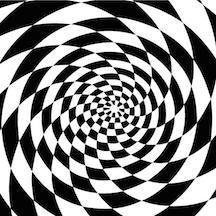
\includegraphics[width=.75\linewidth]{swirl-squares-black-white.jpg}
\caption{Cool checkerboard.}
\label{fig:side-b}
\end{minipage}
\end{figure}

\subsection{Double Quotes.}

Latex double quotes are not the same as the double quote key on your
keyboard. The standard way of writing quotes and double quotes in
LaTeX is with `` and '' not with " and ".   

Now that may be confusing, so you may want to use the \textbackslash\{quotes\} command.  For
example \quotes{The quick brown fox.}



\subsection{Main Body.}

Avoid bad page or column breaks in
your main text, i.e., last line of a paragraph at the top of a
column or first line of a paragraph at the end of a column. If you
begin a new section or sub-section near the end of a column,
ensure that you have at least two (2)  lines of body text on the same
column. 

\section{Outline}  
The following is a possible outline for your paper.
\subsection{Introduction}
\begin{itemize}
\item Motivation and Goal (The goal of this project is...)
\item Overview of challenge and previous work 
\item Approach 
\item Summary of implementation
\item Summary of results
\end{itemize}

\subsection{Problem Background and Related Work}
\begin{itemize}
\item Survey of prior work with similar goals 
\item For each previous approach, explain what has been done and why it does not meet your goal
\end{itemize}

\subsection{Approach}
\begin{itemize}
\item Key novel idea
\item Why it is a good idea
\end{itemize}

\subsection{Implementation}
\begin{itemize}
\item System overview (flow chart of key steps?)
\item Subsection for each step or issue you addressed
\begin{itemize}
\item Problem statement
\item Possible approaches
\item Chosen approach and why
\item Implementaton details
\end{itemize}
\end{itemize}

\subsection{Evaluation}
\begin{itemize}
\item Experiment design...
\item Data...
\item Metrics...
\item Comparisons...
\item Qualitative results...
\item Quantitative results...
\end{itemize}

\subsection{Summary}
\begin{itemize}
\item Conclusions...
\item Limitations...
\item Future work...
\end{itemize}


\section{Ethics}

Your independent work report should abide by the basic standards of scholarly ethics and by Princeton ``academic regulations, which are designed to ensure the integrity of your academic work.~\cite{odoc}'' If you have any doubts about how to cite
other work, how to quote or include text or images from other works, or other issues, please discuss them with your project adviser or with the IW coordinators. 



\bstctlcite{bstctl:etal, bstctl:nodash, bstctl:simpurl}
\bibliographystyle{IEEEtranS}
\bibliography{references}

\end{document}

